\documentclass{ivoa}
\input tthdefs

\usepackage{listings}
\lstloadlanguages{XML,sh,SQL}
\lstset{flexiblecolumns=true,tagstyle=\ttfamily, showstringspaces=False}

\ivoagroup{Edu IG}

\author{Demleitner, M.}
\author{Molinaro, M.}
\author{Ramella, M.}
\author{Iafrate, G.}
\author{Heinl, H.}

\editor{Demleitner, M.}

\SVN$Rev$
\SVN$Date$
\SVN$URL$

\previousversion{First published version}


\title{Educational Resources in the Virtual Observatory}

\begin{document}

\begin{abstract}
Following the spirit of the Virtual Observatory (VO), the production and
provision of services and material to teach VO usage, both for
introducing VO workflows and as an element of a larger astronomy
curriculum, proceeds in a decentralised manner.  This poses at least two
challenges: First, such material needs to be discoverable, ideally in
both source and rendered forms.  Second, resources suitable for use in
outreach and education, targeted at diverse audiences ranging for
pre-school to researchers also need to be discoverable against the
background of tens of thousands resources targeted at research
astronomers.  This document proposes solutions to both of these
challenges.
\end{abstract}


\section{Introduction}

The Virtual Observatory is a complex tool, introducing numerous
technologies not immediately familiar to the average astronomer.
In enabling university level students
and active researchers to fully exploit the VO's capabilities, course
materials and worked-out use-cases have been found an efficient means of
developing the necessary skills both in interactive course situations
like ``VO Days'' and beyond.  
Efficient ways for interested users to locate such
material as well as for VO operators to curate it are highly desirable.

At the same time, advances in technology and 
communications are creating new and exciting 
opportunities for teachers to bring astronomy into their 
classrooms.  As the VO makes science-grade data publicly available and
classroom sets of (suitably) networked PCs are now standard in schools,
exciting projects come within reach of teachers.  To realise these
potentials,
it is necessary to disseminate educational material to help teachers
in preparing classes.  Such material includes documented step-by-step
tutorials, use cases explaining how to perform basic astrophysical research 
using VO tools and resources, and similar exist in various formats and
have been translated in different languages.

Hence, both training professionals for VO exploitation and the provision
of educational material to school teachers and the greater public
require some way of handling metadata on the available material.  Since
the VO has no central body that could curate such a metadata collection
but instead uses a decentralised registry for the similar problem of
service discovery, it seems natural to employ the VO Registry for
metadata management in text resources as well.  This is what the first
part of this document endeavours to do.

In particular in educational settings below university level, however,
it is frequently desirable to, in effect, hide parts of the VO from
users that would provide for overly frustrating experiences (e.g., data
too complex or too unattractive for the general public, or data so
voluminous that consumer-level hardware would fail).  In the second part
of this document, we propose a mechanism through which a specialised
registry could be curated to provide resources specifically selected as
being appropriate for outreach and school-level education.


\section{Registering Texts}

\label{sect:regext}

As argued above, disseminating text-like material
like tutorials, worked-out use cases, or larger introductions,
is an important task in facilitating VO exploitation.  
Within the VO community, there is a large body of
educational material for a wide variety of audiences ranging from pre-school to
researchers.  Existing collections include:

\begin{itemize}

\item EURO-VO AIDA WP5 -- \url{http://wwwas.oats.inaf.it/aidawp5/eng_download.html}

\item EURO-VO Scientific Tutorials -- \url{http://www.euro-vo.org/?q=science/scientific-tutorials}

\item GAVO tutorials --
\url{http://www.g-vo.org/pmwiki/Documents/Tutorials}

\item GAVO's courses on ADQL (\url{http://docs.g-vo.org/adql}) and pvVO
(\url{http://docs.g-vo.org/pyvo})

\item CDS tutorials -- \url{http://cdsweb.u-strasbg.fr/tutorials/}
\end{itemize}


To date, such material has been collected informally by the various
projects on plain web pages as the ones just mentioned.  
It is, in consequence, hard to find, with
knowledge of its existence often passed on anectdotically. In order to improve upon 
this situation, we
propose to keep record of educational material in the VO Registry.

The VO already has a registry extension for standards, which of
course are also text-like: StandardsRegExt \citep{2012ivoa.spec.0508H}.  This extension,
however, focuses on metadata important for standards – e.g.,
vocabularies and status – that is not pertinent for educational
material.  Conversely, it is not concerned with document language (which
can safely be assumed to be English for standards), and it disregards
the issue of locating formatted and source versions, which for educational
material is important.  

Therefore, we believe text-like material should be described in a 
registry extension of its own: DocRegExt.


\subsection{Use Cases}

\label{sect:regext-usecases}

The design of DocRegExt has been guided by the desire to fulfill the
following discovery cases:


\begin{itemize}

\item Is there a tutorial covering discovering intermediate mass black
holes? (Standard VOResource is sufficient){}

\item Is there a tutorial covering working with X-Ray data? (Standard
VOResource is sufficient){}

\item Is there a tutorial dealing with planets suitable for school use?
(Standard VOResource is sufficient){}

\item Is there a tutorial dealing with planets suitable for school use in
Italian? (That requires the declaration of the document language){}

\item What are the subjects of maintained (in the sense of: probably
working in the VO as found by the students) tutorials?
(The active flag of standard VOResource is
unsuitable here since even outdated resources will still be accessible;
we have to get a better idea of how a tutorial would transition into
unmaintained before this use case can actually be supported)

\item Are there tutorials using redshifts? (This is solved by allowing
table metadata in DocRegExt){}

\item Where can I find an editable version of tutorial ivo://auth/tut1?
(This is solved by interfaces with a \xmlel{role} of \textit{source}).

\item Are there translations of tutorial ivo://auth/tut2? (This is
solved by modelling different translations as capabilities of the same
resource).

\item Is there material using service ivo://auth/svc1? (Declaring
standard VOResource relationships covers this use case)

\item Is there material about something visible tonight? (In principle,
allowing the coverage element withing DocRegExt resources enables this
use case, although as of this writing, the Registry infrastructure does
not support spatial discovery).

\item I found this VO tutorial somewhere on the net (``on a mirror'').  Is it
the latest version?  If not, where can I find an update? (Unless the
title of the text changed, standard VOResource should suffice){}

\end{itemize}

An important additional use case is enabling an attractive, browsable
list of registred educational material.  A first attempt at such a
service is GAVO's VO Text Treasures (VOTT)
service\footnote{\url{http://dc.g-vo.org/VOTT}}.  It was found that one
requirement resulting from this use case is direct access to formatted
material in order to enable thumbnail generation.

On the use cases of locating editable forms of such texts – which
has been found to be necessary fairly regularly – we note in passing
that representing source-product relationships is in principle in the
domain of provenance and thus not in the Registry's main scope. However, in
the case discussed here the relation is so simple and its representation
so useful that we propose to include it in a DocRegExt.

\subsection{A Document Registry Extension}

%% NOTE: When you change the schema, make Markus run a 
%% make install-schema
%% to update the current "canonical" schema location.

\label{sect:regext-ext}

To satisfy the requirements derived above, we have designed a registry extension with
two definitions. 
To avoid unnecessary incompatibilities when migrating to a proper IVOA
standard, we use the namespace URI

$$\hbox{\nolinkurl{http://www.ivoa.net/xml/DocRegExt/v1/}}$$

for DocRegExt even while the schema cannot actually retrieved from
there.  The canonical schema location until the extension is endorsed by
the IVOA is \url{http://docs.g-vo.org/xml/DocRegExt/v1/}.

The recommended schema prefix for DocRegExt is \texttt{doc}.

To let authors define comprehensive metadata, the schema
re-uses the \xmlel{vs:CatalogService} type
from VODataService 1.1 \citep{2010ivoa.spec.1202P} to construct
the \xmlel{doc:Document} resource type.  We import the schema by major
version, such that further enhancements within the VODataService version
1 series will apply to DocRegExt records, too.  This in particular
applies to the proposed extensions to declare space-time coverage
\citep{note:regstc}.

While the schema does not limit what kinds of capabilities a
\xmlel{doc:Document} record has -- it is conceivable that tailored
services are communicated in this way --, access to actual files is
enabled using \xmlel{doc:Edition}-typed capabilities.  It may be
argued that this use of VOResource capabilities stretches their
semantics a bit.  We argue, however, that these documents can well be
understood as parameterless service endpoints.  Using capabilities
furthermore allows a complete representation of the metadata in RegTAP
without any extra tables (cf.~sect.~\ref{sect:docregext-regtap}).

The resource-level reference URL in \xmlel{doc:Document} records should
be some sort of landing page with an abstract of the text and links to
the full texts and perhaps the document source(s).  When using the
versioned repository (sect.~\ref{sect:svn-repo}), this could be the
top-level README file within the VCS.  For simple documents, it is
acceptable to use the English-language document itself as
\xmlel{referenceURL}; documents only available in non-English should
provide a landing page with an English-language abstract, though.

The \vorent{facility} and \vorent{instrument} items should only be set
if the text in question actually exploits particular properties of the
concrete instrument.  A \vorent{tableset} can be given for the central
table-like structures a text deals with and facilitates discovery by
physics via the UCDs given in the tableset.

Document-typed resource records should define relations to other
general resources (e.g., applications or services)
they use.  VOResource 1.1 provides a vocabulary of possible
relationships. Document records should preferably use \emph{Cites} and
in particular declare relationships to tools.  If these are not
registred, use the name of their binary as the name of the related
resource; this will very typically be lowercase-only.

Each \xmlel{doc:Edition}-typed capability should 
correspond to a translation of the document.  It
is recommended to list the English-language version first if it exists.

The following description of the \xmlel{doc:Edition} capability
is generated from the schema file.

% GENERATED: !schemadoc DocRegExt-1.0.xsd Edition
\begin{generated}
\begingroup
      	\renewcommand*\descriptionlabel[1]{%
      	\hbox to 5.5em{\emph{#1}\hfil}}\vspace{2ex}\noindent\textbf{\xmlel{doc:Edition} Type Schema Documentation}

\noindent{\small
        An “edition” (typically: translation) of the document.
      \par}

\noindent{\small
        Although for a while, multiple editions of the document in one language
        may be given (corresponding perhaps to two “major” versions), in
        general, only the latest version of the document per language should be
        present.

        At least one vr:WebBrowser-typed interface with 
        role="rendered" must be present. The access URL of the interface
        points to a rendered version of the edition (preferably in PDF, 
        but HTML is acceptable, too).

        Editors are strongly encouraged to also provide an 
        interface with role="source", the accessURL of which should point
        to an editable version of the document, a version controlled
        repository, or the like.
      \par}

\vspace{1ex}\noindent\textbf{\xmlel{doc:Edition} Type Schema Definition}

\begin{lstlisting}[language=XML,basicstyle=\footnotesize]
<xs:complexType name="Edition" >
  <xs:complexContent >
    <xs:extension base="vr:Capability" >
      <xs:sequence >
        <xs:element name="languageCode" type="xs:token" minOccurs="1"
                  maxOccurs="1" />
        <xs:element name="locTitle" type="xs:token" minOccurs="0"
                  maxOccurs="1" />
      </xs:sequence>
    </xs:extension>
  </xs:complexContent>
</xs:complexType>
\end{lstlisting}

\vspace{0.5ex}\noindent\textbf{\xmlel{doc:Edition} Extension Metadata Elements}

\begingroup\small\begin{bigdescription}\item[Element \xmlel{languageCode}]
\begin{description}
\item[Type] string: \xmlel{xs:token}
\item[Meaning] 
                The language this document is (mainly) written in,
                as an BCP 47 language code.
              
\item[Occurrence] required
\item[Comment] 
                The country codes must be given in all lowercase.  This
                results in strings like en, de, or, where regions
                might actually matter, es-es or es-mx.

                This language is also the language for locTitle, 
                irrespective of that element's xml:lang setting.
              

\end{description}
\item[Element \xmlel{locTitle}]
\begin{description}
\item[Type] string: \xmlel{xs:token}
\item[Meaning] 
              	The translated document's title in the language specified
              	by the language sibling.
            	
\item[Occurrence] optional
\item[Comment] 
              	It is recommended to set this element's xml:lang element
              	to the same value as the language sibling.  The reason
              	xml:lang is not used in the first place is that with an
              	extra element, enforcing that the content language is
              	given is more straightforward.
              

\end{description}


\end{bigdescription}\endgroup

\endgroup
\end{generated}

% /GENERATED

\subsection{DocRegExt in RegTAP}
\label{sect:docregext-regtap}

In the relational registry \citep{2014ivoa.spec.1208D}, DocRegExt is
straightforwardly represented in the standard VOResource tables.  in
particular, to find all access urls for documents together with their
English-language titles, one would write:

\begin{lstlisting}[language=SQL]
SELECT res_title, access_url FROM
  rr.resource 
  NATURAL JOIN rr.interface
WHERE
  res_type='doc:document'
  and intf_role='rendered'
\end{lstlisting}

The \xmlel{languageCode} and \xmlel{locTitle} elements from the
\xmlel{doc:Edition} capability extension are mapped into
\verb|res_details| with the following \verb|detail_xpath|s:

\begin{itemize}

\item \texttt{/capability/languageCode} -- the document language as an 
BCP 47 \citep{std:BCP47} language code.
\item \texttt{/capability/locTitle} -- the title in the national
languate.
\end{itemize}

The downside of not defining an extra table for the documents is that
the query patterns in RegTAP are somewhat clumsy.  For instance, to list
the English and Italian titles of all texts available in Italian, one
has to carefully join two subqueries to \verb|res_details|:

\begin{lstlisting}[language=SQL]
SELECT res_title, loctitle FROM
  rr.resource 
  NATURAL JOIN (
    SELECT ivoid, loctitle FROM (
        SELECT ivoid, cap_index, detail_value as loctitle
        FROM rr.res_detail
        WHERE detail_xpath='/capability/locTitle') AS titles
      NATURAL JOIN (
        SELECT ivoid, cap_index 
        FROM rr.res_detail
        WHERE 
          detail_xpath='/capability/languageCode'
          AND detail_value LIKE 'it%') AS italiancaps
    ) as loctitles
WHERE
  res_type='doc:document'
\end{lstlisting}

\subsection{An Example DocRegExt Record}

The following example record corresponds to an actual resource.  It
omits curation information and two of the available languages.  Long
URLs have been wrapped for typographic reasons; of course, in actual
records, no whitespace is allowed within URLs (but since
\xmlel{accessURL} is of type \xmlel{xs:token}, leading and trailing
whitespace is discarded).  Also note that interfaces with
\textit{source} roles
are given for the German and Spanish versions.  This is because the
corresponding files were lost (see sect.~\ref{sect:svn-repo} for a
proposal designed to reduce such problems).

\lstinputlisting[language=XML,basicstyle=\footnotesize]{m1distance-example.xml}

\subsection{A versioned repository for tutorials}

\label{sect:svn-repo}

Registering text documents as VO resources allows searching for tutorials
and similar 
material through standard registry interfaces, but keeping 
tutorials up to date, in their master form and also in their translated 
versions, is an obviously important management issue not really
addressed by the Registry.

For tracking changes and versions, the standard tool is a version
control system.  Therefore,
a versioned repository (using subversion as the version control system) 
has been set up at GAVO data
center\footnote{\url{http://svn.ari.uni-heidelberg.de/svn/edu/}}.
It collects part of the
already existing VO tutorials with the goal of preserving them and
letting users 
update and translate them.

The repository has an internal structure designed to enable:

\begin{itemize}

\item different national languages (master language set to english){}

\item translation vs.~master language updates{}

\item licensing, in order to clarify how and whether a tutorial can be changed or re-used{}

\item additional material used by tutorials

\item access roles to let everyone access tutorials but prevent untrusted updates or additions to it

\end{itemize}

Details of this structure are discussed in a \texttt{README} file at the
root of the
repository\footnote{\url{http://svn.ari.uni-heidelberg.de/svn/edu/README}}.
The repository is intended to work as a space for cooperative 
VO tutorials development.



\section{A Curated Registry for Education}

\label{sect:curreg}


From a technical point of view the registration of educational services
does not require extensions
to the existing for VOResource standard \citep{2008ivoa.spec.0222P}.
The only real need for investigating changes to what already exists
because several
use cases require a distinction particularly suitable for teaching and
outreach
versus resources targeted at professional researchers that might be a
liability in outreach settings.

For simplicity here we will distinguish these two groups of resources as
\emph{educational}
 and 
\emph{professional}
 but without any intent of putting them
on different levels of importance.  In particular, we recognise that the
two sets are not disjunct.



\subsection{Educational vs. Professional Resources}

\label{sect:eduvspro}


On the one side, teachers and educators may find it difficult to filter out 
from all VO resources those that are suitable for their tutorials and
examples. On the other side, educational resources should not be retrieved 
by a standard professional query.
Even allowing that it is not a matter of data quality but rather a distinction on 
the resources' scope, this duality nevertheless poses question as to the
proper way to tag resources for educational usage.
  


In the next subsection we propose a possible tagging solution, based upon 
the existing 
\vorent{ContentLevel}
element of VOResource, but requiring a small change
to it. The subsequent subsection describes the idea of a
curated registry for educational resources and the reasons for it to exist.
  


\subsection{ContentLevel granularity issue}

\label{sect:contentlvl}

VOResource 1.0 already has the 
\vorent{ContentLevel}
element
allowing data publishers to optionally identify their resources as being 
suitable for one or more of the following audiences:


\begin{itemize}

\item General{}

\item Elementary Education{}

\item Middle School Education{}

\item Secondary Education{}

\item Community College{}

\item University{}

\item Research{}

\item Amateur{}

\item Informal Education{}

\end{itemize}

This element turns out to be misused by many publishers, presumably because
it is not really clear what the subtle differences between the available
possibilities are; also, to require a fairly substantial enumeration to
convey ``for school use'' seems, in retrospect, not likely to promote
widespread adoption. We hence propose to simplify the content model
to:


\begin{itemize}

\item General{}

\item Research{}

\item Amateur{}

\end{itemize}

We expect this to reach two goals:
  
\begin{itemize}

\item to make publishers to better describe (on the average)
    their resources{}

\item to providing a tagging solution that suits a first filtering 
    on the resources at client level{}

\end{itemize}

The eventual
addition of an 
\emph{Educational}
value in the list (or perhaps even
substitute it to the 
\emph{General} term with it),
could enhance overall utility of the classification.
  


This change in the already existing standard will require only 
a small effort to update already registered resources because nearly 97\% of 
them currently have \xmlel{contentLevel} set to 
\emph{research}, about 2\% of them have
no \xmlel{contentLevel} defined at all and only the remaining have a different value
(or set of values) set for this element (Appendix \ref{app:clcurrval} details better these
figures).
  

The change proposed here is part of VOResource~1.1, which is in late
public review as this is written.  Even publishing registries not yet
transitioning to VOResource~1.1 are encouraged as
a ``best practice'' to map VOResource~1.0
\vorent{ContentLevel} values 
  of 
\emph{University}
 to 
\emph{Research}
 and
  everything else except 
\emph{Amateur}
 to 
\emph{General}.



\subsection{Curating the Edu Registry}

\label{sect:edureg}

\begin{figure}

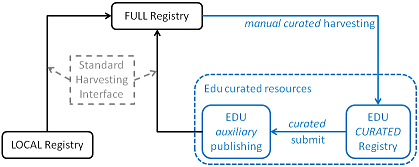
\includegraphics[width=0.9\textwidth]{curation.png}
\caption{Graphic illustration
    of the connecting interfaces between full registries and the educational
    curated one. The 
\emph{auxiliary}
 publishing is the only automatic token
    from the edu part.}
\label{fig:curation}
\end{figure}




Even when the simplified 
\vorent{ContentLevel}
tagging system is in place,
a curated registry for educational VO resources will be useful for
educators in order to let their students work with a registry without having to
worry about confusing material or overwhelming data sizes. A good example
for this is the educational version of the Aladin sky atlas that has a
built-in, curated set of resources suitable for educational level 
tutorials.
  


Curation will require some effort in managing and keeping up to date
such a registry but, most important, it is subject to  some restrictions coming from
the IVOA resource registry architecture. 
  


If such a registry were a standard publishing registry as laid down in
Registry Interfaces
\citep{2009ivoa.spec.1104B},
its resources would be harvested by the full registries: this means 
that any dedicated educational resource would end up in the full VO 
set of resources.  For reasons mentioned above, this is not
desirable.


If it were to be a full registry, it will harvest itself all the existing
resources, and not all of them will fit, or be suitable for, the educational
scope the registry has to be preserved for.
  


What we need is a resource (the curated, in Registry Interfaces
parlance, local, registry) capable of:
  
\begin{itemize}

\item 
\emph{selectively}
 harvesting the existing VO resources 
	(e.g., from a full registry);{}

\item register its own educational resources without being directly
	harvested by full registries (e.g., this could be done using a
	sibling publishing registry dedicated to host those educational
	resources that are to be harvested by the standard full registries.{}

\end{itemize}

This solution, also illustrated in Fig. 1, will not touch the existing architecture
while giving flexibility for the emerging educational resources to 
be curated.
  


\appendix

\section{ContentLevel values summary}

\label{app:clcurrval}

\begin{table}
\begin{tabular}{lp{12cm}}
\sptablerule
\textbf{count}&
\textbf{content\_level string}\\
\sptablerule
  18875 & research\\
  392 & \\
  42 & general university research amateur\\
  31 & general\\
  19 & university research\\
  16 & general university research\\
  9 & university research amateur\\
  8 & research university\\
  4 & amateur research\\
  3 & general research\\
  3 & elementary education middle school education secondary education\\
  3 & research university community college\\
  3 & secondary education community college university research amateur\\
  2 & research general\\
  2 & university\\
  2 & general informal education\\
  2 & elementary education middle school education secondary education community college university research\\
  1 & university community college research\\
  1 & university research amateur informal education\\
  1 & university research general informal education\\
  1 & content\_level\\
  1 & general elementary education middle school education secondary education community college university research amateur informal education\\
  1 & general university research informal education\\
  1 & elementary education middle school education secondary education community college university research amateur informal education\\
  1 & research amateur general\\
  1 & research amateur informal education\\
  1 & elementary education middle school education secondary education community college university research amateur\\
  1 & research university amateur\\
\sptablerule
\end{tabular}
\caption{Empirical distribution of \vorent{ContentLevel}s declared by VO
resources.}
\label{tab:cldist}
\end{table}

This appendix reports some statistics on the usage of the ContentLevel 
element in \citep{2008ivoa.spec.0222P} as of 2018-02-26, taken from the
GAVO RegTAP endpoint at \url{http://reg.g-vo.org/tap}.
There were 19427 useful resources (excluding authorities, standards and
similar) that expose 28 different values as their ContentLevel.
In table \ref{tab:cldist} these values are reported in order of count.

Up-to-date numbers from the same endpoint (or an analogue 
one) can be obtained by using the following ADQL query:

\begin{verbatim}
SELECT 
  count(*) as cnt, content_level
FROM 
  rr.resource
WHERE
  res_type not in ('vstd:servicestandard', 'vg:authority', 
    'vstd:standard', 'va:application', 'vr:organization')
GROUP BY content_level
ORDER BY cnt DESC
\end{verbatim}

The table shows that less than 1\% of the ContentLevel values 
are different from
\emph{research}, when 
the element is not empty. Morever, of the 160 ``non-trivial'' resources,
100 include the \emph{general} value (63\% of them), 
only 3 (2\%) state that are devoted to some 
\emph{education} level only,
while 148 (90\%) state that are also devoted to some 
\emph{education} level (up to 
\emph{university}).

\section{Changes}

\subsection{Changes from 1.0}

\begin{itemize}
\item Following XML itself, we now ask for BCP 47 rather than RFC
3066 language codes.
\end{itemize}

\bibliography{ivoatex/ivoabib,ivoatex/docrepo}

\end{document}
